% !TEX root = main.tex
% !TEX root = main.tex
\documentclass[12pt]{report}
\usepackage[utf8]{inputenc}

% Formatting
\usepackage[mmddyyyy]{datetime}
\usepackage{fullpage}
\usepackage{enumerate}

%\usepackage{subfiles}

\usepackage{xargs}
\usepackage{xparse}


% Math util stuff
\usepackage{amsmath}
\usepackage{amsthm}
\usepackage[makeroom]{cancel}

\usepackage{pgfplots}
\pgfplotsset{compat=newest}
\pgfplotsset{
    axis lines=middle,
    axis line style={<->},
    every axis plot post/.append style={mark=none,samples=200,smooth},
    unit vector ratio=1 1 1
}

\everymath{\displaystyle}

% Theorem styling
\theoremstyle{plain}
\newtheorem{theorem}{Theorem}[section]
\newtheorem{corollary}{Corollary}[theorem]
\newtheorem{lemma}[theorem]{Lemma}
\newtheorem{review}{Review}[section]

\theoremstyle{definition}
\newtheorem{definition}{Definition}[section]
\newtheorem{example}{Example}[theorem]

\theoremstyle{remark}
\newtheorem*{remark}{Remark}
\newtheorem*{note}{Note}

\DeclareMathOperator{\di}{d\!}

\newcommandx*\deriv[2][1=, 2=x, usedefault]{\dfrac{\di {#1}}{\di {#2}}}

\DeclareDocumentCommand \Eval { m m O{} } { \left.#1\right\rvert_{#2}^{#3} }

\renewcommand{\partname}{Chapter}

% \usepackage{showframe}

\title{
    Calculus I Notes\\
    \large MATH 1190}
\author{Logan Thompson}
\date{}

\begin{document}
\hypersetup{pageanchor=false}
\maketitle
\hypersetup{pageanchor=true}
\tableofcontents
\newpage
\chapter*{Introduction}
\section*{What is this?}
This is a project to keep all of my notes for my Calculus I class in a nice PDF file.
\section*{About this project}
This PDF is created using a combination of \LaTeX\ and Wolfram Mathematica. All code for this project can be found on its \href{https://github.com/Cobbleopolis/Calculus-Notes}{GitHub page}. This project is intended to be built on a Windows computer because it relies on running a \texttt{.bat} file at compile time.

Also, if any errors are found in the PDF please create an issue on this project's GitHub page \href{https://github.com/Cobbleopolis/Calculus-Notes/issues}{here}. This includes any errors in the math or spelling or grammar errors as my editor that I use for this project does not have spell check.

Pull requests and controbutions are wlecome.
\stepcounter{chapter}
\chapter{The Derivative}
% !TEX root = ../main.tex

\section{Rates of Change and The Derivative}
A particle's rectilinear (1D) motion has its position defined by the function $s(t) = 5 - t^2$, where $s$ is measured in meters and $t$ in seconds.
\begin{enumerate}
    \item Sketch the graph of the function on the interval from $t = 0$ to $t = 4$.
    \item Find the \textit{average} velocity over the time over the time interval from $t = 0$ to $t = 4$. On your graph, draw what this quantity represents.
    \item Approximate the \textit{instantaneous} velocity when $t = 2$ by finding the average velocity over the intervals $t = 2$ to $t = 3$, $t = 2$ to $t = 2.5$, and $t = 2$ to $t = 2.1$.
    \item Write a general expression that represents the average velocity over the time interval from $t = 2$ to $t = 2 + h$.
    \item Find the instantaneous velocity when $t = 2$ by finding the limit of the above expression as $h \to 0$.
\end{enumerate}
Answers:
\begin{enumerate}
    \item \leavevmode\vadjust{\vspace{-\baselineskip}}\newline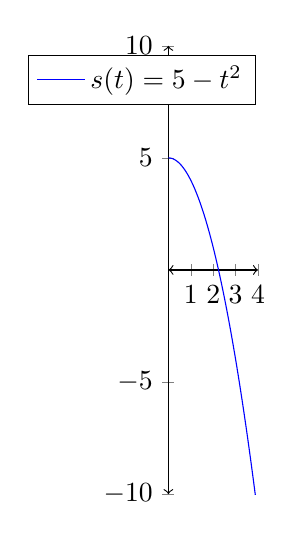
\begin{tikzpicture}
    \begin{axis}[xmin=0, xmax=4, ymin=-10, ymax=10]
        \addplot+ {5 - x^2};
        \legend{$s(t) = 5 - t^2$};
    \end{axis}
    \end{tikzpicture}
    \item \begin{gather*}
        \dfrac{\Delta s}{\Delta t} \\
        \dfrac{s(4) - s(0)}{4 - 0} \\
        \dfrac{\left(5 - 4^2 \right) - \left(5 - 0^2\right)}{4} \\
        \dfrac{-11 - 5}{4} \\
        -4 [m/s]
    \end{gather*}
    \item \begin{itemize}
        \item $t = 2$ to $t = 3$:\begin{gather*}
            \dfrac{s(3) - s(2)}{3 - 2} \\
            \dfrac{\left(5 - 3^2\right) - \left(5 - 2^2\right)}{1} \\
            -5 [m/s]
        \end{gather*}
        \item $t = 2$ to $t = 2.5$:\begin{gather*}
            \dfrac{s(2.5) - s(2)}{3 - 2} \\
            \dfrac{\left(5 - 2.5^2\right) - \left(5 - 2^2\right)}{0.5} \\
            -4.5 [m/s]
        \end{gather*}
        \item $t = 2$ to $t = 2.1$:\begin{gather*}
            \dfrac{s(2.1) - s(2)}{3 - 2} \\
            \dfrac{\left(5 - 2.1^2\right) - \left(5 - 2^2\right)}{0.1} \\
            -4.1 [m/s]
        \end{gather*}
        \textit{Guess:} velocity \underline{at} $t = 2$ is approximately $4[m/s]$.
    \end{itemize}
    \item \begin{gather*}
        \dfrac{s(2 + h) - s(2)}{2 + h - 2} \\
        \dfrac{\left(5 - \left(2 + h\right)^2\right) - \left(5 - 2^2\right)}{h} \\
        \dfrac{5 - \left(4 + 4h + h^2\right) - \left(1\right)}{h} \\
        \dfrac{-4h - h^2}{h} \\
        -4 - h
    \end{gather*}
    \item \begin{gather*}
        \lim_{h \to 0} \left(\dfrac{s(2 + h) - s(2)}{h}\right) \\
        \lim_{h \to 0} \left(-4 - h\right) \\
        -4 - 0 \\
        -4
    \end{gather*}
\end{enumerate}
\subsection{Definitions}
The slope of a curve can be found using the following equations:
\begin{equation}
    \lim_{x \to c} \left(\dfrac{f(x) - f(c)}{x - c}\right)
\end{equation}
\begin{equation}
    \lim_{h \to 0} \left(\dfrac{f(c + h) - f(c)}{h}\right)
\end{equation}
These are also known as:
\begin{itemize}
    \item The \textit{instantaneous} velocity of an object at time $c$ whose position is given by the function $f(x)$.
    \item The \textit{slope of the tangent line} to the curve $y = f(x)$ at $x = c$.
    \item The \textit{instantaneous rate of change} of the function $f(x)$ at $x = c$.
    \item The \textit{derivative} of $f$ at $c$.
    \item $f'(c)$
\end{itemize}
\begin{example}
    Find the slope of the line tangent to $y = \dfrac{1}{x + 5}$ when $x = 1$. Then find the equation for the tangent line at that point.
    \begin{gather*}
        \lim_{h \to 0} \left(\dfrac{f(1 + h) - f(1)}{h}\right) \\
        \lim_{h \to 0} \left(\dfrac{\dfrac{1}{1 + h + 5} - \dfrac{1}{1 + 5}}{h}\right) \\
        \lim_{h \to 0} \left(\dfrac{\left(\dfrac{6}{6} \cdot \dfrac{1}{1 + h + 5}\right) - \left(\dfrac{1}{1 + 5} \cdot \dfrac{6 + h}{6 + h}\right)}{h}\right) \\
        \lim_{h \to 0} \left(\dfrac{\dfrac{6}{6\left(6 + h\right)} - \dfrac{6 + h}{6\left(6 + h\right)}}{h}\right) \\
        \lim_{h \to 0} \left(\dfrac{\dfrac{-h}{6\left(6 + h\right)}}{h}\right) \\
        \lim_{h \to 0} \left(\dfrac{1}{\cancel{h}} \cdot \dfrac{-\cancel{h}}{6\left(6 + h\right)}\right) \\
        \lim_{h \to 0} \left(\dfrac{-1}{6\left(6 + h\right)}\right) \\
        \dfrac{-1}{36}
    \end{gather*}
    Equation of line: We have the slope, all we need is a point (substitute $1$ in for $x$).
    \begin{gather*}
        y = \dfrac{1}{1 + 6}\\
        y = \dfrac{1}{6}
    \end{gather*}
    So the point is $(1, \dfrac{1}{6})$.
    Equation:
    \begin{gather*}
        y - \dfrac{1}{6} = -\dfrac{1}{36} \left(x - 1\right) \\
        y = -\dfrac{1}{36}x + \dfrac{1}{36} + \dfrac{1}{6} \\
        y = -\dfrac{1}{36}x + \dfrac{7}{36} \\
    \end{gather*}
\end{example}
% TODO Add slide 11

% !TEX root = ../main.tex

\section{The Derivative of a Function}
\begin{theorem}[Derivative]
    The derivative of $f$ is the function
    \begin{equation}
        f'(x) = \lim_{h \to 0}\left(\dfrac{f\left(x + h\right) - f(x)}{h}\right)
    \end{equation}
\end{theorem}
\begin{remark}
    This is only true if the limit exists.
\end{remark}
\begin{corollary}
    If the limit does exist at $x=c$ then $f$ is differentiable at $c$
\end{corollary}
\begin{corollary}
    If the limit exists at every point in interval $\left[a, b\right]$ then $f$ is differentiable on $\left[a, b\right]$. \\
    \includegraphics{Chapter2/Section2/test.pdf}
\end{corollary}
\begin{example}
    If $f(x) = x^2 + 2x + 1$ find $f'(x)$.
    \begin{align*}
        f'(x) &= \lim_{h \to 0}\left(\dfrac{f\left(x + h\right) - f(x)}{h}\right) \\
        f'(x) &= \lim_{h \to 0}\left(\dfrac{\left(\left(x+h\right)^2 + 2\left(x + h\right) +1 \right) - \left(x^2 + 2x + 1\right)}{h}\right)\\
        f'(x) &= \lim_{h \to 0}\left(\dfrac{\cancel{x^2} + 2xh + h^2 + \cancel{2x} + 2h + \cancel{1} - \cancel{x^2} - \cancel{2x} - \cancel{1}}{h} \right) \\
        f'(x) &= \lim_{h \to 0}\left( \dfrac{2xh + h^2 + 2h}{h} \right) \\
        f'(x) &= \lim_{h \to 0}\left( 2x + h + 2 \right) \\
        f'(x) &= 2x + 2
    \end{align*}
\end{example}
\begin{example}
    Let $f(x) = \sqrt{x}$. Find $f'(x)$.
    \begin{align*}
        f'(x) &= \lim_{h \to 0}\left( \dfrac{f\left(x + h\right) - f(x)}{h} \right) \\
        f'(x) &= \lim_{h \to 0}\left( \dfrac{\sqrt{x + h} - \sqrt{x}}{h} \right)\\
        f'(x) &= \lim_{h \to 0}\left( \dfrac{\sqrt{x + h} - \sqrt{x}}{h} \cdot \dfrac{\sqrt{x+h} + \sqrt{x}}{\sqrt{x+h} + \sqrt{x}} \right)\\
        f'(x) &= \lim_{h \to 0}\left( \dfrac{\cancel{x} + h - \cancel{x}}{h \left(\sqrt{x + h} + \sqrt{x}\right)} \right)\\
        f'(x) &= \lim_{h \to 0}\left( \dfrac{\cancel{h}}{\cancel{h} \left(\sqrt{x + h} + \sqrt{x}\right)} \right)\\
        f'(x) &= \lim_{h \to 0}\left( \dfrac{1}{\sqrt{x + h} + \sqrt{x}} \right)\\
        f'(x) &= \dfrac{1}{\sqrt{x + 0} + \sqrt{x}}\\
        f'(x) &= \dfrac{1}{2\sqrt{x}}\\
    \end{align*}
\end{example}
\begin{corollary}
    Functions will fail to be differentiable at
    \begin{itemize}
        \item Cusps
        \item Corners
        \item Vertical Tangents
        \item Any point where it is discontinuous
    \end{itemize}
\end{corollary}
\begin{lemma}
    If $f$ is differentiable at $x=c$ then $f$ is continuous at $c$. However a function can be continuous but not differentiable (e.g. $y=\left|x\right|$ at $x=0$).
\end{lemma}

% !TEX root = ../main.tex

\section{The Derivative of Polynomial Functions and $y = e^x$}
Recall that if $f(x) = x^2 + 2x + 1$, then $f'(x) = 2x + 2$. We could write this in different ways.
\begin{itemize}
    \item If $y = x^2 + 2x + 1$ then $y' = 2x + 2$.
    \item If $y = x^2 + 2x + 1$ then $\deriv[y] = 2x + 2$.
    \item If $y = x^2 + 2x + 1$ then $\deriv \left(x^2 + 2x + 1\right) = 2x + 2$.
\end{itemize}
\begin{remark}
    The last one, $\deriv$ is an instruction to take a derivative of what comes after it.
\end{remark}
\begin{theorem}[Derivative of a Constant]
    If $A$ is a constant and $f(x) = A$ then $f'(x) = 0$.
\end{theorem}
\begin{theorem}[Derivative of a line with a slope of 1]
    If $f(x) = x$ then $f'(x) = 1$.
\end{theorem}
\begin{review}
    Use the definition of a derivative to find $\deriv \left(x^2\right)$.
    \begin{gather*}
        \lim_{h \to 0}\left(\dfrac{\left(x + h\right)^2 - x^2}{h}\right) \\
        \lim_{h \to 0}\left(\dfrac{x^2 + h^2 + 2xh - x^2}{h}\right) \\
        \lim_{h \to 0}\left(\dfrac{h^2 + 2xh}{h}\right) \\
        \lim_{h \to 0}\left(h + 2x\right) \\
        0 + 2x \\
        2x
    \end{gather*}
\end{review}
\subsection{Basic Rules}
\subsubsection{Power Rule}
\begin{theorem}[Power Rule]
    If $n \geq 1$ is an integer, then
    \begin{align}
       \deriv \left(x^n\right) &= nx^{n-1} \\
       \deriv \left(Cx^n\right) &= (C \cdot n)x^{n-1} \qquad \text{If $C$ is a constant.}
    \end{align}
\end{theorem}
\begin{review}
    If $y = 5x^2$ find $y'$ using the definition of a derivative.
    \begin{align*}
        f'(x) &= \lim_{h \to 0} \left(\dfrac{5\left(x + h\right)^2 - 5x^2}{h}\right) \\
        f'(x) &= \lim_{h \to 0} \left(\dfrac{5\left(\left(x + h\right)^2 - x^2\right)}{h}\right) \\
        f'(x) &= \lim_{h \to 0} \left(\dfrac{5\left(x^2 + h^2 + 2xh - x^2\right)}{h}\right) \\
        f'(x) &= 5\lim_{h \to 0} \left(\dfrac{x^2 + h^2 + 2xh - x^2}{h}\right) \\
        f'(x) &= 5\lim_{h \to 0} \left(\dfrac{h^2 + 2xh}{h}\right) \\
        f'(x) &= 5\lim_{h \to 0} \left(h + 2x\right) \\
        f'(x) &= 5 \cdot 2x \\
        f'(x) &= 10x \\
    \end{align*}
\end{review}
\subsubsection{Constant Multiplication Rule}
\begin{theorem}[Constant Multiplication Rule]
    Suppose $F(x) = k \cdot f(x)$ for some real number $k$ if $f(x)$ is differentiable then $F(x)$ is also differentiable, and
    \begin{equation}
        F'(x) = k \cdot f'(x)
    \end{equation}
\end{theorem}
\begin{example}
    If $f(x) = \pi x^7$ find $f'(x)$.
    \begin{align*}
        f'(x) &= \pi \deriv \left(x^7\right) \\
        f'(x) &= \pi \cdot \left(7x^6\right) \\
        f'(x) &= 7\pi x^6
    \end{align*}
\end{example}
\subsubsection{Addition Rule}
\begin{theorem}[Addition Rule]
    If $F(x) = f(x) + g(x)$ and $f$ and $g$ are differentiable then $F(x)$ is also differentiable.
    \begin{equation}
        F'(x) = f'(x) + g'(x)
    \end{equation}
\end{theorem}
\begin{example}
    If $y=3x^5 - 7x^2 - \dfrac{1}{2}x + 5$ find $\deriv[y]$
    \begin{align*}
        y' &= 3 \cdot \deriv \left(x^5\right) - 7 \cdot \deriv \left(x^2\right) - \dfrac{1}{2} \deriv \left(x\right) + \deriv \left(5\right)\\
        y' &= 3 \cdot 5x^4 - 14x - \dfrac{1}{2} \cdot 1 + 0 \\
        y' &= 15x^4 - 14x - \dfrac{1}{2}
    \end{align*}
\end{example}
\subsection{Derivative of $f(x) = e^x$}
\begin{theorem}[Derivative of $f(x) = e^x$]
    \begin{equation}
        \deriv\left(e^x\right) = e^x
    \end{equation}
    If $f(x) = e^x$, then $f'(x) = e^x$.
\end{theorem}

% !TEX root = ../main.tex

\section{Product Rule, Quotient Rule, and Higher Order Derivatives}
\subsection{Basic Rules Continued}
\subsubsection{Product Rule}
\begin{theorem}[Product Rule]
    If $f$ and $g$ are differentiable then
    \begin{equation}
        \deriv\left(f(x) \cdot g(x)\right) = f(x) \cdot \deriv \left(g(x)\right) + \deriv \left(f(x)\right) \cdot g(x)
    \end{equation}
    Restated:
    \begin{equation}
        \left(f \cdot g\right)' = f \cdot g' + f' \cdot g
    \end{equation}
\end{theorem}
\begin{example}
    If $f(x) = e^xx^4$ find $f'(x)$.
    \begin{align*}
        f'(x) &= e^x \cdot 4x^3 + x^4 \cdot e^x \\
        f'(x) &= 4e^xx^3 + e^xx^4 \\
        f'(x) &= e^xx^3(4 + x) \\
    \end{align*}
\end{example}
\begin{example}
    If $y=4(x^2 - 7)$, find $y'$.
    \begin{align*}
        f'(x) &= 4x^2 - 28 \\
        f'(x) &= 8x
    \end{align*}
\end{example}
\subsubsection{Quotient Rule}
\begin{theorem}[Quotient Rule]
    If $f$ and $g$ are differentiable at $x$ and $g(x) \neq 0$ then $\dfrac{f}{g}$ is differentiable at $x$ and
    \begin{equation}
        \deriv\left(\dfrac{f(x)}{g(x)}\right) = \dfrac{g(x) \cdot \deriv\left(f(x)\right) - f(x) \deriv\left(g(x)\right)}{g(x)^2}
    \end{equation}
    Restated:
    \begin{equation}
        \left(\dfrac{f}{g}\right)' = \dfrac{g \cdot f' - f \cdot g'}{g^2}
    \end{equation}
\end{theorem}
\begin{remark}
    The order of the quotient rule can be remembered with the rhyme ``hi d lo lo d hi all over the square of what's below''.
\end{remark}
\begin{example}
    Find $\deriv\left(\dfrac{3x^3 - 5x}{5e^x+2}\right)$
    \begin{align*}
        f' &= 9x^2-7 \\
        g' &= 5e^x
    \end{align*}
    \begin{equation*}
        \deriv\left(\dfrac{3x^3 - 5x}{5e^x+2}\right) = \dfrac{\left(5e^x + 2\right) \left(9x-7\right) - \left(3x^3 - 7x\right)\left(5e^x\right)}{\left(5e^x + 2\right)^2}
    \end{equation*}
\end{example}
\begin{remark}
    In some cases it is okay to not simplify the answer.
\end{remark}
\subsection{Revising the Power Rule}
\begin{align*}
    f(x)  &= x^n       & f(x)  &= Ax^n \\
    f'(x) &= nx^{x- 1} & f'(x) &= Anx^{n-1}
\end{align*}
Where $n$ is \underline{any} integer.
\begin{example}
    Find $f'(x)$ if $f(x) = \dfrac{1}{3x^4}$.
    \begin{align*}
        f(x) &= \dfrac{1}{3x^4} \\
        f(x) &= \dfrac{1}{3} x^{-4} \\
        f(x) &= -\dfrac{4}{3} x^{-5}
    \end{align*}
\end{example}
\subsection{Higher Order Derivatives}
\begin{definition}
    The derivative if $f'$ is the second derivative of $f$.

    \quad Notation: $f''(x)$

    \quad Read: ``$f$ double prime of $x$''

    \quad Can also consider third derivative $f'''$, fourth derivatives $f^{(4)}$, etc.
\end{definition}
\begin{example}
    If $f(x) = 5x^3$, find $f'$, $f''$, and $f'''$
    \begin{align*}
        f'(x) &= 15x^2 \\
        f''(x) &= 30x \\
        f'''(x) &= 30
    \end{align*}
\end{example}
\subsubsection{Why do we care?}
We know $f'(x)$ tells us the rate of change of $f$. What does $f''(x)$ tell us?
\begin{itemize}
    \item Rate of change of the rate of change...
    \item In the context of $f = \text{position}$:
    \begin{itemize}
        \item $f'$ is velocity (how fast the position is changing)
        \item $f''$ is acceleration (how fast the velocity is changing)
    \end{itemize}
    \item In the context of $f = \text{number of unemployed people in the U.S.}$:
    \begin{itemize}
        \item $f'$ is how quickly unemployment is growing or shrinking
        \item Suppose we are in a recession where unemployment is increasing. As $f''$ decreases, it means that jobs are being more slowly.
    \end{itemize}
\end{itemize}
\begin{example}
    A rock thrown vertically from the surface of the moon at an initial velocity of 24 [m/s] reaches a height of $s = 24t - 0.8t^2$ meters in $t$ seconds
    \begin{enumerate}
        \item What is the velocity at time $t$? What is the acceleration?
        \item How long before the rock reaches its highest point?
        \item How high does the rock go?
        \item How long before the rock reaches half of it's maximum height?
        \item How long is the rock aloft?
        \item What is the rock's speed on impact?
    \end{enumerate}
    Answers:
    \begin{enumerate}
        \item \begin{align*}
            v &= s' = 24 - 16t [m/s] \\
            a &= s'' = -1.6 [m/s^2]
        \end{align*}
        \item \begin{align*}
            24 - 1.6t &= 0 \\
            24 &= 1.6t \\
            t &= 15 [s]
        \end{align*}
        \item \begin{gather*}
            24\left(15\right) - 0.8 \left(15\right)^2 \\
            180[m]
        \end{gather*}
        \item \begin{gather*}
            90 = 24\left(t\right) - 0.8\left(t\right)^2 \\
            0 = -0.8t^2 + 24t - 90 \\
            \dfrac{-24 \pm \sqrt{576 - 4 \cdot -0.8 \cdot -90}}{-1.6} \\
            \dfrac{-24 \pm \sqrt{288}}{-1.6} \\
            \dfrac{-24 \pm 12\sqrt{2}}{-1.6} \\
            t = \underline{4.3934}, 25.6066
        \end{gather*}
        \item $30 [s]$ (Two times the time to reach the peak (see \#2)
        \item $-24 [m/s]$ (Same as initial velocity but negative)
    \end{enumerate}
\end{example}

% !TEX root = ../main.tex
% chktex-file 36

\section{The Derivative of Trigonometric Functions}
Looking at the graph of $y=\sin(x)$, Can we get an idea of how the derivative looks? \\
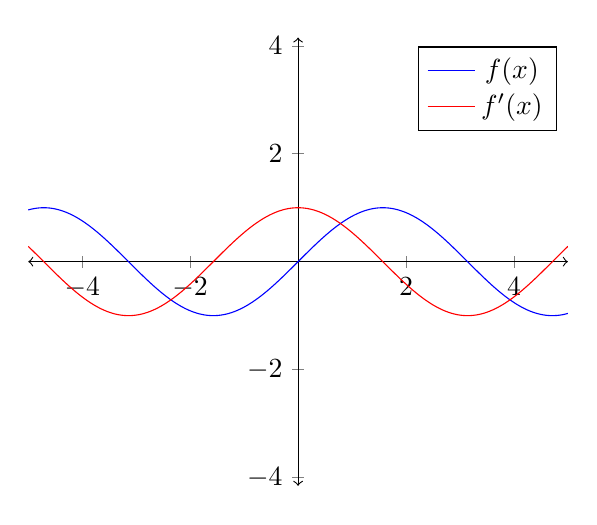
\begin{tikzpicture}
    \begin{axis}
        \addplot+ {sin(deg(x))};
        \addplot+ {cos(deg(x))};
        \legend{$f(x)$, $f'(x)$};
    \end{axis}
\end{tikzpicture}
The derivative of $y = \sin(x)$ is $y' = \cos(x)$
\subsection{Derivatives of \texorpdfstring{$f(x) = \sin(x)$}{f(x) = sin(x)} and \texorpdfstring{$f(x) = \cos(x)$}{f(x) = cos(x)}}
\begin{align}
    \deriv \left(\sin(x)\right) &= \cos(x) \\
    \deriv \left(\cos(x)\right) &= -\sin(x)
\end{align}
\begin{example}
    Find $\deriv \left(x\cos(x)\right)$
    \begin{align*}
        \deriv \left(x\right) &= 1 \\
        \deriv \left(\cos(x)\right) &= -\sin(x)
    \end{align*}
    \begin{gather*}
        x \cdot \deriv \left(\cos(x)\right) + \deriv \left(x\right) \cdot \cos(x) \\
        x \left(-\sin(x)\right) + 1 \cdot \cos(x) \\
        -x\sin(x) + \cos(x)
    \end{gather*}
\end{example}
\subsection{Derivative of \texorpdfstring{$f(x) = \tan(x)$}{f(x) = tan(x)} }
\begin{equation}
    \deriv \left(\tan(x)\right) = \sec^2(x)
\end{equation}
\begin{proof}
    Proof that $\deriv\left(\tan(x)\right) = \sec^2(x)$.
    \begin{gather*}
        \deriv \left(\tan(x)\right) = \deriv \left(\dfrac{\sin(x)}{\cos(x)}\right) \\
        \dfrac{\cos(x) \cdot \cos(x) - \sin(x) \cdot - \sin(x)}{\cos^2(x)} \\
        \dfrac{\cos^2(x) + \sin^2(x)}{\cos^2(x)} \\
        \dfrac{1}{\cos^2(x)} \text{\quad -OR- \quad} 1 + \tan^2(x) \\
        \sec^2(x)
    \end{gather*}
\end{proof}
\begin{example}
    Find the derivative of $y = \cot(x)$ in two ways: Using $sin(x)$ and $cos(x)$, and using $tan(x)$. \\
    Method 1:
    \begin{gather*}
        \deriv\left(\dfrac{\cos(x)}{\sin(x)}\right) \\
        \dfrac{\sin(x) \cdot -\sin(x) - \cos(x) \cdot \cos(x)}{\sin^2(x)} \\
        \dfrac{-\sin^2(x) - \cos^2(x)}{\sin^2(x)} \\
        \dfrac{-\left(\sin^2(x) + \cos^2(x)\right)}{\sin^2(x)} \\
        -\dfrac{1}{sin^2(x)} \\
        -\csc^2(x)
    \end{gather*}
    Method 2:
    \begin{gather*}
        \deriv\left(\dfrac{1}{\tan(x)}\right) \\
        \dfrac{\tan(x) \cdot \deriv\left(1\right) - 1 \cdot \deriv\left(\tan(x)\right)}{\tan^2(x)} \\
        \dfrac{\cancel{\tan(x) \cdot 0} - \sec^2(x)}{\tan^2(x)} \\
        -\dfrac{\sec^2(x)}{\tan^2(x)} \\
        \dfrac{\dfrac{1}{\cancel{\cos^2(x)}}}{\dfrac{\sin^2(x)}{\cancel{\cos^2(x)}}} \\
        -\dfrac{1}{\sin^2(x)} \\
        -\csc^2(x)
    \end{gather*}
\end{example}
\subsection{Derivatives of SIX basic trig functions}
\begin{align}
    \deriv \left(\sin(x)\right) &= \cos(x) \\
    \deriv \left(\cos(x)\right) &= -\sin(x) \\
    \deriv \left(\tan(x)\right) &= \sec^2(x) \\
    \deriv \left(\cot(x)\right) &= -\csc^2(x) \\
    \deriv \left(\sec(x)\right) &= \sec(x)\tan(x) \\
    \deriv \left(\csc(x)\right) &= -\csc(x)\cot(x)
\end{align}

\chapter{More About Derivatives}
% !TEX root = ../main.tex

\section{The Chain Rule}
Suppose we have
\begin{equation*}
    f(x) = \sin(x^2)
\end{equation*}
It is a composite function
\begin{gather*}
    g(x) = \sin(x) \\
    h(x) = x^2 \\
    g(h(x)) = f(x) \\
    (g \circ h)(x) = f(x)
\end{gather*}
\subsection{The Chain Rule}
\begin{note}
    This is helpful in Calculus II
\end{note}
\begin{theorem}
    Suppose we have $f$ and $g$ are both differentiable then
    \begin{equation}
        \left(f \circ g\right)' = f'(g(x)) \cdot g'(x)
    \end{equation}
\end{theorem}
\begin{example}
    \begin{align*}
        f(x) &= \sin(x^2) \\
        f'(x) &= \cos(x^2) \cdot 2x
    \end{align*}
\end{example}
\begin{example}
    \begin{gather*}
        y = \tan^2(\theta) \\
        y = \left(\tan(\theta)\right)^2
    \end{gather*}
    \begin{align*}
        f(x)      &= x^2          & f'(x)      &= 2x \\
        g(\theta) &= \tan(\theta) & g'(\theta) &= \sec^2(\theta)
    \end{align*}
    \begin{equation*}
        y' = 2\left(\tan(\theta)\right) \cdot \sec^2(\theta)
    \end{equation*}
\end{example}
\begin{example}
    \begin{equation*}
        s(x) = \csc(\cos(x))
    \end{equation*}
    \begin{align*}
        f(x) &= \csc(x) & f'(x) &= -\csc(x)\cot(x) \\
        g(x) &= \cos(x) & g'(x) &= -\sin(x)
    \end{align*}
    \begin{gather*}
        s'(x) = -\csc(\cos(x))\cot(\cos(x)) \cdot -\sin(x) \\
        s'(x) = \sin(x)\csc(\cos(x))\cot(\cos(x))
    \end{gather*}
\end{example}
\begin{example}\hspace{\textwidth}\\
    a): find y'
    \begin{equation*}
        y = \left(\dfrac{3x^2 + 1}{2x^2 - x}\right)^4
    \end{equation*}
    \begin{align*}
        f(x) &= x^4                        & f'(x) &= -\csc(x)\cot(x)\\
        g(x) &= \dfrac{3x^2 + 1}{2x^2 - x} & g'(x) &= \dfrac{-3x^2 - 4x + 1}{\left(2x^2 - x\right)^2}
    \end{align*}
    \begin{gather*}
        y' = 4\left(\dfrac{3x^2 + 1}{2x^2 - x}\right)^3\left(-\dfrac{3x^2 - 4x + 1}{\left(2x^2 - x\right)^2}\right) \\
        y' = \dfrac{-4 \left(3x^2 + 1\right)^3\left(3x^2 + 4x - 1\right)}{\left(2x^2 - x\right)^5}
    \end{gather*}
    b) Find where the curve has horizontal tangents. (y' = 0)
    \begin{gather*}
        \dfrac{-4 \left(3x^2 + 1\right)^3\left(3x^2 + 4x - 1\right)}{\left(2x^2 - x\right)^5} = 0 \\
        -4 \left(3x^2 + 1\right)^3\left(3x^2 + 4x - 1\right) = 0 \\
        \cancel{-4 = 0} \qquad \text{no solutions} \\
        3x^2 + 1 = 0 \qquad \text{no solutions} \\
        3x^2 + 4x - 1 = 0 \\
        x = \dfrac{-4 \pm \sqrt{16 -4\left(3\right)\left(-1\right)}}{2\left(3\right)} \\
        x = \dfrac{-4 \pm \sqrt{38}}{6}
    \end{gather*}
\end{example}
\begin{example}
    \begin{gather*}
        y = \left(x\right)\left(\sec(e^x)\right) \\
        y' = x \cdot \deriv \left(\sec(e^x)\right) + \deriv \left(x\right) \cdot \left(\sec(e^x)\right) \\
        y' = x \cdot \sec(e^x)\tan(e^x) \cdot \deriv\left(e^x\right) + \deriv \left(x\right) \cdot \left(\sec(e^x)\right) \\
        y' = x \cdot e^x \sec(e^x) \tan(e^x) + \deriv \left(x\right) \cdot \left(\sec(e^x)\right) \\
        y' = x \cdot e^x \sec(e^x) \tan(e^x) + 1 \cdot \left(\sec(e^x)\right) \\
        y' = \sec(e^x)\left(x e^x \tan(e^x) + 1\right)
    \end{gather*}
    \begin{note}
        Do you chain rule or product rule ``first''? It depends!
    \end{note}
\end{example}
\subsection{Constant to the Power of \texorpdfstring{$x$}{x} Rule}
We want to derive $y = 3^x$. \\
Start by writing $3^x$ in terms of $e^x$:
\begin{gather*}
    3^x = e^{\ln(3^x)} \\
    3^x = e^{x\ln(3)}
\end{gather*}
Use the chain rule:
\begin{align*}
    f(x) &= e^x     & f'(x) &= e^x \\
    g(x) &= x\ln(3) & g'(x) &= \ln(3)
\end{align*}
\begin{gather*}
    y' = e^{x\ln(3)} \cdot \ln(3) \\
    y' = 3^x \cdot \ln(3)
\end{gather*}
\begin{theorem}[Constant to the Power of $x$ Rule]
    If we assume that $a$ is constant where $a > 0$ and $a \neq 1$ then:
    \begin{equation}
        \deriv \left(a^x\right) = a^x \cdot \ln(a)
    \end{equation}
\end{theorem}
\begin{example}
    \begin{equation*}
        y = 2^{x^5}
    \end{equation*}
    \begin{align*}
        f(x) &= 2^x & f'(x) &= 2^x \cdot \ln(2) \\
        g(x) &= x^5 & g'(x) &= 5x^4
    \end{align*}
    \begin{gather*}
        y' = 2^{x^5} \ln(2) \cdot 5x^4 \\
        y' = 5 \cdot \ln(2) \cdot x^4 \cdot 2^{x^5}
    \end{gather*}
\end{example}
\begin{example}
    \begin{gather*}
        y = 3 \sec(2^x) \\
        y' = 3 \deriv \left(\sec(2^x)\right)
    \end{gather*}
    \begin{align*}
        f(x) &= \sec(x) & f'(x) &= \sec(x)\tan(x) \\
        g(x) &= 2^x     & g'(x) &= 2^x \cdot \ln(2)
    \end{align*}
    \begin{gather*}
        f'(x) = 3 \sec(2^x) \tan(2^x) \cdot 2^x \ln(2) \\
        f'(x) = \left(3 \ln(2)\right)2^x \sec(2^x) \tan(2^x)
    \end{gather*}
\end{example}

% !TEX root = ../main.tex

\section{Implicit Differentiation}
Some curves' equations can't be solved for y (or maybe not easily), but we should still be able find the tangent line and its slope.
\begin{example}
    \begin{equation*}
        x^2 + y^2 = 4
    \end{equation*}
    \begin{itemize}
        \item Not a function!
        \item Can solve for $y$
    \end{itemize}
    \begin{equation*}
        y = \pm \sqrt{4 - x^2}
    \end{equation*}
    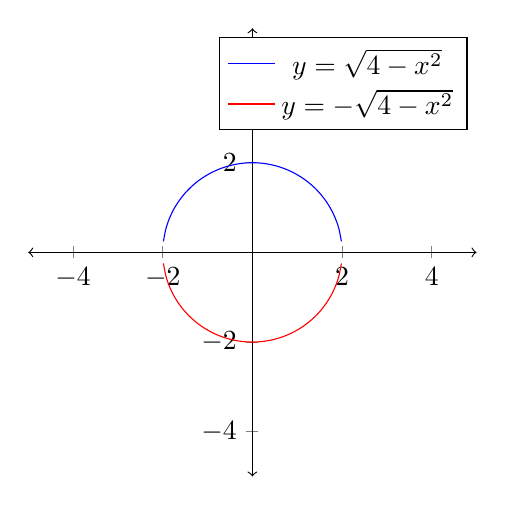
\begin{tikzpicture}
        \begin{axis}[xmin = -5, xmax=5, ymin=-5, ymax=5]
            \addplot +[blue]{sqrt(4 - x^2)};
            \addplot +[red]{-sqrt(4 - x^2)};
            \legend{$y = \sqrt{4 - x^2}$, $y = -\sqrt{4 - x^2}$};
        \end{axis}
    \end{tikzpicture}\\
    Given an expression with $x$s and $y$s to find $\deriv[y]$
    \begin{enumerate}
        \item Treat $y$ as a function of $x$ and differentiate both sides of the equation with respect to $x$
        \item Solve for $\deriv[y]$
        \item Win
    \end{enumerate}
    \begin{note}
        When doing step one (1), you can thing ``Whenever I thake the derivative of $y$ multiply that term by $\deriv[y]$.''
    \end{note}
    \begin{example}
        If $x^2 + y^2 = 4$ use implicit differentiation to find $\deriv[y]$
        \begin{enumerate}[a)]
            \item \begin{gather*}
                \deriv \left(x^2 + y^2\right) = \deriv \left(4\right) \\
                2x + 2y\deriv[y] = 0 \\
                \dfrac{\cancel{2y}\deriv[y]}{\cancel{2y}} = \dfrac{-2x}{2y} \\
                \deriv[y] = \dfrac{-2x}{2y} \\
                \deriv[y] = -\dfrac{x}{y}
            \end{gather*}
            \item Find the slope of the tangent line at $\left(1, \sqrt{3}\right)$ \\
            \begin{equation*}
                \Eval{\deriv[y]}{\left(1, \sqrt{3}\right)} = - \dfrac{1}{\sqrt{3}}
            \end{equation*}
            \begin{note}
                The line after $\deriv[y]$ is read as ``$\deriv[y]$ evaluated with $ x= 1$ and $y = \sqrt{3}$''
            \end{note}
            \item What is the equation of the tangent at $\left(1, \sqrt{3}\right)$
            \begin{gather*}
                y - y_1 = m\left(x - x_1\right) \\
                y - \sqrt{3} = - \dfrac{1}{\sqrt{3}}\left(x - 1\right)
            \end{gather*}
        \end{enumerate}
    \end{example}
    %TODO complete Section 3.2
\end{example}

% !TEX root = ../main.tex

\section{Derivatives of Logarithmic Functions}
\begin{theorem}[Derivatives of Logarithmic Functions]
    If we recall that $\log_a(x) = y$, then $a^y = x$ as well as $\deriv\left(a^x\right) = a^x \ln(a)$ then the following must be true:
    \begin{equation}
        \deriv \left(\log_a(x)\right) = \dfrac{1}{x\ln(a)}
    \end{equation}
\end{theorem}
\begin{proof}
    \begin{align*}
        \log_a(x) &= y \\
        a^y &= x \\
        \deriv \left(a^y\right)    &= \deriv \left(x\right)\\
        a^y \ln(a) \cdot \deriv[y] &= 1 \\
        \deriv[y]                  &= \dfrac{1}{a^y \ln(a)} \\
        \intertext{This is fine but we don't want $y$ in our answer.}
        \deriv[y]                  &= \dfrac{1}{x \ln(a)} \\
        \intertext{This is valid because we know that $a^y = x$}
    \end{align*}
\end{proof}
What about $\deriv\left(\ln(x)\right)$?
\begin{align*}
    \deriv\left(\ln(x)\right) &= \deriv \left(\log_e(x)\right) \\
                              &= \dfrac{1}{x\ln(e)} \\
                              &= \dfrac{1}{x}
\end{align*}
\begin{note}
    The power rule will never give an exponent of $-1$, since $n = 0$ would mean that it's a constant.
\end{note}
\begin{example}
    Differentiate: $f(x) = \dfrac{x}{\ln(x)}$
    \begin{align*}
        f'(x) &= \dfrac{\left(\ln(x)\right)\deriv\left(x\right) - \left(x\right)\deriv\left(\ln(x)\right)}{\left(\ln(x)\right)^2} \\
              &= \dfrac{\left(\ln(x)\right)\left(1\right) - \left(x\right)\left(\dfrac{1}{x}\right)}{\left(\ln(x)\right)^2} \\
              &= \dfrac{\ln(x) - 1}{\left(\ln(x)\right)^2} \\
              &= \dfrac{\ln(x)}{\left(\ln(x)\right)^2} - \dfrac{1}{\left(\ln(x)\right)^2} \tag{Optional} \\
              &= \dfrac{1}{\ln(x)} - \dfrac{1}{\left(\ln(x)\right)^2} \tag{Optional}
    \end{align*}
\end{example}
\begin{example}
    Differentiate $y = \left|x\right|$
    \begin{equation*}
        y = \begin{cases}
            \ln(x) & x > 0 \\
            \ln(-x) & x < 0
        \end{cases}
    \end{equation*}
    \begin{note}
        Domain is all real number except 0
    \end{note}
    \begin{align*}
        x  &> 0:           & x &< 0: \\
        y  &= \ln(x)       & y &= \ln(-x) \\
        y' &= \dfrac{1}{x} & y' &= \dfrac{1}{-x} \cdot \deriv \left(-x\right) \\
           &               & y' &= \dfrac{1}{-x} \left(-1\right) \\
           &               &    &= \dfrac{1}{x}
    \end{align*}
    Conclusion: because $y'$ was the same in both cases then the following must be true:
    \begin{equation*}
        \deriv\left(\ln(\left|x\right|)\right) = \dfrac{1}{x}
    \end{equation*}
\end{example}
%TODO Finish section 3.3

% !TEX root = ../main.tex

\section{Newton's Method}
How do we solve equations like $x^3 - 4x + 2 = 0$?
\begin{itemize}
    \item We could use a calculator\ldots But what about before calculators? And HOW do calculators solve it?
    \item We could factor it. But factoring polynomials of high degrees really isn't fun. Maybe it doesn't factor (i.e. $\sin^2(x) + 2x - 5$)
    \item There are a variety of \textit{numerical methods} that calculators and computers use to find roots of equations.
    \item One such method id Newton's Method.
\end{itemize}
\subsection{Intermediate Value Theorem}
\begin{theorem}[Intermediate Value Theorem]
    If $f$ is continouts on $[a, b]$ and $N$ is between $f(a)$ and $f(b)$, then there is some $c \in (a, b)$ such that $f(c) = N$.
    \begin{note}
        $c \in (a, b)$ means that the value $c$ is between $a$ and $b$
    \end{note}
    \includegraphics[scale=0.75]{Chapter3/Section4/ivtGraph.pdf}\\
\end{theorem}
\subsection{The idea behind Newtom's Method}
Suppose $f(x)$ is a polynomial.
\begin{itemize}
    \item Suppose we can apply the IVT to conclude that $f$ has a root between $a$ and $b$.
    \item We pick any value, $c_1$, between $a$ nd $b$, and use that as our first guess of what the zero might be.
    \item We probably won't be right because there are an infinite amount of numbers between $a$ and $b$.
    \item We can evaluate $f(c_1)$ using a calculator.
    \item We can find $f'(c_1)$ because we are awesome at derivatives\ldots right?
\end{itemize}
Because $c_1$ is an approximation and is probably wrong we need to be able to ge a more accruate estimate. To do that we take the tangent line of $f(c_1)$ and where it intersects the x-axis is $c_2$. Repeat the process to get a progressively more and more accurate estimate for the root of the function.
\begin{center}
    \includegraphics{Chapter3/Section4/newtonsMethod.pdf}
\end{center}
\subsection{A Recursive Formula}
If $c_1$ is our first estimate the we can get a better approximation $c_2$ (called the ``second approximation'') by finding
\begin{equation*}
    c_2 = c_1 - \dfrac{f(c_1)}{f'(c_1)}
\end{equation*}
The third approximation is
\begin{equation*}
    c_3 = c_2 - \dfrac{f(c_2)}{f'(c_2)}
\end{equation*}
We can keep going to get the $n$th approximation
\begin{equation}
    c_n = c_{n - 1} - \dfrac{f(c_{n - 1})}{f'(c_{n - 1})}
\end{equation}
\begin{note}
    In \textit{most} cases when computers (calculators, laptops, etc.) are asked to find the square root of a function they actually use Newton's Method to find the square root. For example, if we asked a computer to find $\sqrt{S}$ it would have the function $f(x) = x^2 - S$ and then applies Newton's Method to find the square root of $S$. In fact, \textit{most} processors have an instruction that is used to take the square root of a number and the most common implementation of this instruction uses Newton's Method and it is accurate up to 5 bits.
\end{note}
\begin{example}
    Verify that $f(x) = x^3 - 4x + 2$ has a root on the interval $(1, 2)$. Then use a first approximation of $c_1 = 1.5$ to find the third approximation of that root.
    \begin{gather*}
        f(1) = 1^3 - 4(1) + 2 = -1 \\
        f(2) = 2^3 - 4(2) + 2 = 2
    \end{gather*}
    The IVT says that this function \textit{must} have a root in $(1, 2)$.
    \begin{equation*}
        f'(x) = 3x^2 - 4
    \end{equation*}
    \begin{gather*}
        c_2 = c_1 - \dfrac{f(c_1)}{f'(c_2)} \\
        c_2 = 1.5 - \dfrac{f(1.5)}{f'(1.5)} \\
        c_2 = 1.5 - \dfrac{(1.5)^3 - 4(1.5) + 2}{3(1.5)^2 - 4} \approx 1.727
    \end{gather*}
    \begin{equation*}
        c_3 = 1.727 - \dfrac{(1.727)^3 - 4(1.727) + 2}{3(1.727)^2 - 4} \approx 1.678
    \end{equation*}
    The actual root is approximately 1.675, so we're correct up to two decimal places in just two iterations.
\end{example}
\begin{example}
    Verify that $f(x) = x^4 - x^3 + x - 2$ has a root on the interval $(1, 2)$. Then use a first approximation of $c_1 = 1.5$ to find the fourth approximation of that root.
    \begin{gather*}
        f(1) = 1^4 - 1^3 + 1 - 2 < 0 \\
        f(2) = 2^4 - 2^3 + 2 - 2 > 0
    \end{gather*}
    The IVT says that this function \textit{must} have a root in $(1, 2)$.
    \begin{equation*}
        f'(x) = 4x^3 - 3x^2 + 1
    \end{equation*}
    \begin{gather*}
        c_2 = c_1 - \dfrac{f(c_1)}{f'(c_1)} \\
        c_2 = 1.5 - \dfrac{(1.5)^4 - (1.5)^3 + 1.5 - 2}{4(1.5)^3 - 3(1.5)^2 + 1} \\
        c_2 \approx 1.3468
    \end{gather*}
    \begin{gather*}
        c_3 = c_2 - \dfrac{f(c_2)}{f'(c_2)} \\
        c_3 = 1.3468 - \dfrac{(1.3468)^4 - (1.3468)^3 + 1.3468 - 2}{4(1.3468)^3 - 3(1.3468)^2 + 1} \\
        c_3 \approx 1.3104
    \end{gather*}
    \begin{gather*}
        c_4 = c_3 - \dfrac{f(c_3)}{f'(c_3)} \\
        c_4 = 1.3104 - \dfrac{(1.3104)^4 - (1.3104)^3 + 1.3104 - 2}{4(1.3104)^3 - 3(1.3104)^2 + 1} \\
        c_4  \approx 1.3086
    \end{gather*}
    This is actually correct up to 4 decimal places!
\end{example}
\subsection{Good News and Bad News}
\subsubsection{Bad News}
Sometimes Newton's Method fails. For example, your $c_1$ might be at a point where there is a horizontal tangent and it won't intersect the x-axis
\subsubsection{Good News}
It doesn't fail very often, and when it works, it gets close to the right answer ``very quickly.''

\chapter{Applications of the Derivative}
% !TEX root = ../main.tex

\section{Related Rates}
Problem asks for a rate of change of some quantity; use the rate of change of related quantities.
\begin{example}
    The volume of a right circular cone is given by
    \begin{equation*}
        V = \dfrac{1}{3}\pi r^2h
    \end{equation*}
    How does the volume change over time with respect to the change in height if $r$ is constant?
    \begin{align*}
        \deriv[][t]\left(V\right) &= \deriv[][t]\left(\dfrac{1}{3}\pi r^2 h\right) \\
        1 \cdot \deriv[V][t] &= \underbrace{\dfrac{1}{3}\pi r^2}_\text{constant} \cdot 1 \cdot \deriv[h][t]
    \end{align*}
    How is $\deriv[V][t]$ related to $\deriv[r][t]$ if h is constant?

\end{example}
\subsection{Practice}
If a snowball melts so that its surface area decreases at a rate of \SI{1}{\cm\squared\per\min}, find the rate at which the diameter decreases when the diameter is \SI{10}{\cm}. (Surface area of a sphere: $SA = 4\pi r^2$)\\
\begin{tikzpicture}
    \draw[<->] (0,3) -- (6,3) node[midway, above] {d};
    \draw(3, 3) circle (3 cm);
\end{tikzpicture}
\subsubsection{Solution}
Variables we know:
\begin{align*}
    d &= \text{ diameter} \\
    SA &= \text{ surface area} \\
    \deriv[SA][t] &= \SI{1}{\cubic\cm\per\min}
\end{align*}
Variables we want:
\begin{equation*}
    \Eval{\deriv[d][t]}{d = \SI{10}{\cm}}
\end{equation*}
Equation:
\begin{align*}
    SA &= 4\pi r^2\\
    SA &= 4\pi \left(\dfrac{d}{2}\right)^2 \\
    SA &= \pi d^2
\end{align*}
Derive:
\begin{equation*}
    \deriv[SA][t] = \pi \cdot 2d \cdot \deriv[d][t]
\end{equation*}
Substitute:
\begin{gather*}
    \SI{1}{\cm\squared\per\min} = \pi \cdot 2\left(\SI{10}{\cm}\right) \cdot \deriv[d][t] \\
    \deriv[d][t] = \dfrac{\SI{-1}{\cm\squared\per\min}}{\SI{20\pi}{\cm}} \\
    \deriv[d][t] = \dfrac{-1}{20\pi}\text{ }\SI{}{\cm\per\min}
\end{gather*}
The diameter is decreasing at $\dfrac{-1}{20\pi}\text{ }\SI{}{\cm\per\min}$

% !TEX root = ../main.tex

\placeholderSection{Maximum and Minimum Values}

% !TEX root = ../main.tex

\placeholderSection{The Mean Value Theorem}

% !TEX root = ../main.tex

\placeholderSection{Local Extrema and Concavity}

% !TEX root = ../main.tex

\section{Indterminate Forms and L'Hopital's Rule}
\subsection{Indeterminate Forms}
Let's look at the first two forms we're going care about here.\\
If
\begin{equation*}
    \lim_{x \to c}\left(f(x)\right) = \lim_{x \to c}\left(g(x)\right) = 0
\end{equation*}
then $\dfrac{f(x)}{g(x)}$ is an indeterminate form of the type $\dfrac{0}{0}$.\\
If
\begin{equation*}
    \lim_{x \to c}\left(f(x)\right) = \lim_{x \to c}\left(g(x)\right) = \infty
\end{equation*}
then $\dfrac{f(x)}{g(x)}$ is an indeterminate form of the type $\dfrac{\infty}{\infty}$.
\begin{note}
    $c = \infty$ is allowed
\end{note}
View these cases as we get \textit{no information} when we substitute to try and find the limit.
\begin{example}
    Evaluate: $\lim_{x \to 0}\left(\dfrac{\tan(x)}{x}\right)$ \\
    Remember:
    \begin{equation*}
        \lim_{x \to 0}\left(\dfrac{\sin(\theta)}{\theta}\right) = 1
    \end{equation*}
    \begin{gather*}
        \lim_{x \to 0}\left(\dfrac{\tan(x)}{x}\right) \subeq \dfrac{0}{0} \\
        \lim_{x \to 0}\left(\dfrac{\dfrac{\sin(x)}{\cos(x)}}{x}\right) \\
        \lim_{x \to 0}\left(\dfrac{\sin(x)}{x} \cdot \dfrac{1}{\cos(x)}\right) \\
        \lim_{x \to 0}\left(\dfrac{\sin(x)}{x}\right) \cdot \lim_{x \to 0}\left(\dfrac{1}{\cos(x)}\right)\\
        1 \cdot \dfrac{1}{1}\\
        1
    \end{gather*}
\end{example}
\subsection{L'Hopital's Rule}
\begin{theorem}[L'Hopital's Rule]
    Suppose $f$ and $g$ are differentiable near $c$, and $g'(x) \neq 0$ for all $x \neq c$ near $c$. Let $L$ be a real number (or $\pm \infty$), and suppose $\dfrac{f(x)}{g(x)}$ in an indeterminate form at $c$ of type $\dfrac{0}{0}$ or $\dfrac{\infty}{\infty}$. If
    \begin{equation}
        \lim_{x \to c}\left(\dfrac{f'(x)}{g'(x)}\right) = L
    \end{equation}
    then
    \begin{equation}
        \lim_{x \to c}\left(\dfrac{f(x)}{g(x)}\right) = L
    \end{equation}
\end{theorem}
The rule basically says \textbf{if you satart with a $\dfrac{0}{0}$ or $\dfrac{\infty}{\infty}$ indterminate form}, then taking the derivative of the top and the derivative of the bottom will not change the limit.\\
We are \textbf{NOT} taking the derivative of $\dfrac{f(x)}{g(x)}$!. Never take the derivative of a quotient without using the quotient rule.\\ %TODO reference quotient rule
You many need to apply the rule multiple times. You might get another indeterminate form when you take the derivative; so apply the rule again.\\
\textbf{YOU HAVE TO START WITH AN INDETERMINATE FORM!}
\begin{example}
    Evaluate: $\lim_{x \to 0}\left(\dfrac{\tan(x)}{x}\right)$ \\
    \begin{align*}
        \lim_{x \to 0}\left(\dfrac{\tan(x)}{x}\right) &\subeq \dfrac{0}{0} \\
        &\lheq \lim_{x \to 0}\left(\dfrac{\sec^2(x)}{1}\right) \\
        &\subeq \dfrac{\sec^2(0)}{1} \\
        &= \dfrac{1}{1} \\
        &= 1
    \end{align*}
    \begin{note}
        The ``L'H'' in $\lheq$ is required so we know that L'Hopital's Rule was used.
    \end{note}
    \begin{note}
        It is \textbf{NOT} true that $\dfrac{\tan(x)}{x} = \dfrac{\sec^2(x)}{1}$, so you really need the limit opperator to keep the staments equivelent.
    \end{note}
\end{example}

% !TEX root = ../main.tex

\placeholderSection{Curve Sketching}

% !TEX root = ../main.tex

\placeholderSection{Optimization}

% !TEX root = ../main.tex

\placeholderSection{Antiderivative; Differential Equations}

\chapter{The Integral}
% !TEX root = ../main.tex

\placeholderSection{Area}

% !TEX root = ../main.tex

\placeholderSection{The Definite Integral}

% !TEX root = ../main.tex

\placeholderSection{The Fundamental Theroem of Calculus}

\appendix
% !TEX root = ../main.tex

\chapter{Buddy Chart}
\begin{align*}
  \deriv\left(x^n\right) &= nx^{n-1}\\
  \deriv\left(a^x\right) &= a^x\ln(a) \\
  \deriv\left(e^x\right) &= e^x \\
  \deriv\left(\sin(x)\right) &= \cos(x) \\
  \deriv\left(\cos(x)\right) &= -\sin(x) \\
  \deriv\left(\tan(x)\right) &= \sec^2(x) \\
  \deriv\left(\csc(x)\right) &= -\csc(x)\cot(x) \\
  \deriv\left(\sec(x)\right) &= \sec(x)\tan(x) \\
  \deriv\left(\cot(x)\right) &= -\csc^2(x) \\
  \deriv\left(\sin^{-1}(x)\right) &= \dfrac{1}{\sqrt{1 - x^2}} \\
  \deriv\left(\cos^{-1}(x)\right) &= -\dfrac{1}{\sqrt{1 - x^2}} \\
  \deriv\left(\tan^{-1}(x)\right) &= \dfrac{1}{1 + x^2} \\
  \deriv\left(\csc^{-1}(x)\right) &= -\dfrac{1}{x\sqrt{x^2-1}} \\
  \deriv\left(\sec^{-1}(x)\right) &= \dfrac{1}{x\sqrt{x^2-1}} \\
  \deriv\left(\cot^{-1}(x)\right) &= -\dfrac{1}{1 + x^2} \\
  \deriv\left(\log_a(x)\right) &= \dfrac{1}{x\ln(a)} \\
  \deriv\left(\ln(x)\right) &= \dfrac{1}{x}
\end{align*}

\end{document}
